\documentclass[11pt]{article}

\usepackage{geometry}                % See geometry.pdf to learn the layout options. There are lots.
\geometry{letterpaper}                   % ... or a4paper or a5paper or ... 
%\geometry{landscape}                % Activate for for rotated page geometry
%\usepackage[parfill]{parskip}    % Activate to begin paragraphs with an empty line rather than an indent
\usepackage{graphicx}
\usepackage{amssymb}
\usepackage{epstopdf}
%\usepackage{enumitem}
\usepackage{ulem}
\DeclareGraphicsRule{.tif}{png}{.png}{`convert #1 `dirname #1`/`basename #1 .tif`.png}
\usepackage{caption}
\usepackage{subcaption}

\title{Siderope O-ring Remediation}
\author{Ryan Bayes}
\date{\today; V4}

\begin{document}
\maketitle
\section{Introduction}
The side rope boxes are a part of the SNO+ calibration system  consisting of four large motor boxes each containing the rope spools coupled to an external motor, and connected to the UI through a 1/2 inch tube by way of one of four load cell boxes. As such, they are integrated into the SNO+ UI cover gas space.  Two of the motor boxes, the North Motor box and East Load Cell box seals have not shown leaks with a vacuum leak checker in excess of $10^{-4}$ mbar L/s where the expectation is that the leak should be less than $10^{-7}$ mbar L/s. Problems have also been observed in both the South motor box and load cell boxes. The results of the previous leak checking campaigns are shown in table \ref{tab:leakCheck}.

	\begin{table}
	\caption{Summary of previous leak checking campaigns as applied to the calibration side rope systems}
	\label{tab:leakCheck} 
	\begin{center}
	\begin{tabular}{|r|c|c|c|}
	\hline
	Feature & Status & Leak (mbar L/s)& Date\\\hline
	East and west motor box & good & $< 2\times10^{-8}$ & June 2023 \\
	West load cell box seal & good & $< 10^{-10}$ & June 2023 \\
	South motor box outer seal & pass & $5\times10^{-7}$ & June 2023 \\
	South motor box inner seal & fail &  $1.4\times10^{-5}$ & July 2023 \\
	South exten. box outer seal & fail &  $< 10^{-5}$ & June 2023 \\
	South exten. box inner seal & pass &  $2\times10^{-9}$ & July 2023 \\
	North motor box & fail &  $ > 10^{-4}$ & Oct 2019 \\
	North load cell box & pass&  $ < 10^{-9}$ & June 2023 \\
	East load cell box seal & fail & $ > 10^{-4}$ & Oct 2019 \\
	\hline
	\end{tabular}
	\end{center}
	\end{table}
	
Plastic bags flushed with nitrogen have been put over the boxes and this has reduced the radon levels somewhat, but the current background load in the detector is not reasonable. For this reason a more active approach to correcting this problem must be taken. The hypothesis is that there is something wrong with one or both of the o-rings that constitute the motor box seals. To remedy this problem the o-rings must be inspected and, if necessary, replaced. This procedure outlines the methods needed to conduct an o-ring inspection and replacement in a way that reduces radon ingress into the detector as much as possible.

\section{Definitions}
\begin{itemize}
\item {\bf AV}; Acrylic Vessel - The centre of the SNO+ detector containing the active scintillator volume
\item {\bf AV neck} - A 7 metre long cylinder that connects to the spheroidal main body of the AV. 
\item {\bf UI}; Universal interface - The cap on the top of the AV neck consisting of the lower UI through which tubes for recirculation and extracting samples from the AV are connected, and the upper UI through which ports for gas lines, level sensors and calibration equipment exist. 
\item {\bf DCR}; Deck clean room - a tent in the centre of the SNO+ deck to isolate activities about the UI that may introduce contamination into the experiment from the rest of the lab. Is equipped with multiple hepa filters to circulate and clean the air that passes into the facility. 
\item {\bf Bubblers} - Three gas lines that run into the UI through a bubbler flange which use gas pressure to determine the fluid level in the AV. 
\item {\bf Neck tubes} - PMTs installed on the UI to veto events suspected of appearing in the neck. Contained in steel top-hats with a coaxial electrical feedthrough on top. 
\item {\bf Radon monitor} - A 3 m$^{3}$ vacuum vessel used to measure levels of radon daughters in the cover gas volume. It is connected to the UI cover gas through a 1" diameter bellows hose. 
\item {\bf Side rope motor box} - One of four boxes cantilevered off of the UI. Used to adjust the tension on the ropes used to guide sources in a 2-dimensional plane in the UI (either XZ or YZ). Necessarily connected to the UI cover gas through a 1/2" tube containing the side rope. All four motor boxes are equipped with quick connects to facilitate a clean connection to the UI cover gas space.
\item {\bf Side rope load cell box} - One of four boxes used to align the side rope with a feed through to enter the UI. So called because the original design called for a load cell to be included to provide a secondary measurement of the rope tension. The load cell is not connected into the manipulator system, however. Each load cell box is connected to the siderope motor box via a 1/2" inch tube with VCR connections on both ends. Each is further connected to the UI cover gas through the rope feedthrough. Two load cell boxes (East and South) are equipped with valves to allow for clean connections to the UI cover gas.  
\end{itemize}

\begin{figure}[htbp]
\begin{center}
\includegraphics[width=0.8\textwidth]{UIView.png}
\caption{The UI with pink plastic nitrogen bags installed on the UI over the North Motor Box and the East Load cell box.}
\label{fig:UI}
\end{center}
\end{figure}


\begin{figure}[htbp]
\begin{center}
\includegraphics[width=0.5\textwidth]{EastropeWindow.png}
\caption{One of the motor boxes with an acrylic window installed to see the interior mechanisms.}
\label{fig:eastrope}
\end{center}
\end{figure}

section{Personnel}
\begin{itemize}
\item Task Lead: Ryan Bayes
\item Second: Matt Depatie
\item Cover gas expert: Aleksandra Bialek
\item Cover gas monitor: Parmesh Ravi (training required)
\end{itemize}


\section{Parts and Equipment List}
\begin{itemize}
	\item 2$\times$ TEV o-ring; 604mm $\times$ 2.6 mm
	\item 2$\times$ TEV o-ring; 596mm $\times$ 2.6 mm
	\item 2$\times$ TEV o-ring; 456mm $\times$ 2.6 mm
	\item 2$\times$ TEV o-ring; 449mm $\times$ 2.6 mm
	\item 88 hex cap screws for Motor box replacements 20mm $\times$ 1/4", ultrasonically cleaned
	\item 1 (or more) 3/16" Allen key
	\item 1 ratchet with 3/16" hex bit
	\item 1 1/4" torx hex bit (for removing stripped cap screws)
	\item 1 vice grip
	\item 1 mallet
	\item Helium leak checker
	\item Helium spray bottle (filled)
	\item Nitrogen source
	\item Flow meter
	\item Nitrogen regulator
\end{itemize}


\section{Risks and Mitigation}

The risk to workers through this procedure is extremely low. Workers should conduct themselves with the following considerations 
\begin{itemize}
\item  A potential oxygen deprivation hazard due to  exposure to the cover gas. This can be mitigated by ensuring that workers keep their faces well away from open ports to the UI at all times (low risk, low severity)
\item Workers must be aware of pinch points as the purpose of the activity requires sealing heavy metal steel surfaces against each other. (medium risk, low severity)
\item The lids to the motor boxes are heavy, so steps to prevent musculo-skeletal distress should be taken (get help as required and potentially using mechanical assistance if necessary). (medium risk, low severity)
\end{itemize}

\subsection{Radon Mitigation}\label{ss:radmit}
The primary risks with these procedures are to the detector itself through radon ingress. The solution to this is to set up a monitored UI flushing path. This involves
	\begin{enumerate}
	\item Connect one of the load cell gas ports (the valve on the South or East load cell boxes) to a nitrogen source (preference is for a nitrogen bottle) through a regulator and a flow meter with a shut-off valve inside the DCR.
	\item Connect an outflow line using a quick connect, a 1/4" teflon line and a 1/4" check valve and a pump.
	\item Start monitoring the cover gas bag size and UI dp using Delta V. This should be done by a user not directly doing the work on the UI with a laptop situated in the DCR garage.
	\item Start the nitrogen flow into the UI with a pressure less than 10 psi, and a flow less than 5 L/min
	\item Match the nitrogen inflow with the pump outflow pressure. The UI dp must be in a range of $\pm$ 0.05 psi as read out on delta V using DPT-005. Adjustments to the dp should be made by using the valve before the flow meter to throttle the gas flow.
	\item Continue monitoring the UI dp through the UI procedures.
	\item The nitrogen flow should continue for 30 minutes after the motor box is closed and sealed.
	\item Turn off the nitrogen flow followed by the pump in close sequence.
	\item Disconnect the pump from the motor box and move to the next motor box. 
	\end{enumerate}
To reduce the volume that can be exposed to contamination the radon monitor and UI cover gas bags should both be valved off. Both valves are metal seated valves, the operation of which requires a properly set and calibrated torque wrench as part of the closing procedure. The specifications for both are recorded on the valves themselves. 


\section{Procedure}

\subsection{Pre-Requisites}
To conduct this procedure the environment must be prepared. This includes
	\begin{itemize}
	\item The DCR must be well cleaned. This includes vacuuming the floors, wiping down the DCR walls, and wiping down surfaces including shelves and UI
	\item Pass swipe tests on surfaces in the DCR such as the UI, shelving, and URMs.
	\item A benchmark of fewer than 200, 0.5$\mu$m dust counts per $m^{3}$ per second must be achieved in the DCR air.
	\item Prepare all tools for use in a secure location away from the UI, preferably on a trolley for ease of access. This includes wiping down all tools to reduce the chance of dust getting into the UI, ensuring that the required machine screws are available, and wiping down the o-rings.
	\end{itemize}
These cleaning activities and tests must be done on the days prior and the day of the procedure. If at any point the tests fail, cleaning should be redone, and the tests should be done again. 

On the day of the o-ring replacement, the o-rings themselves should have a liberal amount of vacuum grease applied to help them stick in the o-ring grooves during installation.

\subsection{Emergency Procedures}

If there is an all stations call with a side-rope box open
\begin{itemize}
\item Place a cover (the remnants of the North box nitrogen bag should be sufficient) over the open box to provide a dust shield.
\item Change the nitrogen inflow to use a dewar (if using a bottle, switch to using the international). 
\item Maintain the nitrogen flow and monitor it from refuge through the all stations call
\end{itemize}

If there is an all stations call with a side-rope box cover partially in place (i.e. subset of screws installed) or between o-ring replacement procedures. 
\begin{itemize}
\item Change the nitrogen inflow to use a dewar (if using a bottle, switch to using the international). 
\item Maintain the nitrogen flow and monitor it from refuge through the all stations call
\end{itemize}

Assess the situation at the end of the all stations, and determine if work can resume, or if the UI must be put into a safe state (i.e. Cover-gas bags reconnected) until next the working day.

\subsection{Evaluate and Replace North Motor Box Seals}

\newcounter{northcounter}
\newcommand\north{\stepcounter{northcounter}\thenorthcounter}

\begin{tabular}{|c|c|p{15cm}|}
\hline
\north & & Turn off the radon monitor pump and valve off the radon monitor recirculation line. Disconnect the radon monitor return line from the East motor box. Valve off the radon monitor from the UI using the valve on the West side of the radon monitor. \\
\hline\north& & Place the detector at low voltage. \\
\hline\north & & Stop the flow into the UI nitrogen bags. Remove the bags from North motor box and East load cell box.\\
\hline\north & & Connect N$_{2}$ source to UI to "flush" UI as described in subsection \ref{ss:radmit}. The in-flow line should be connected to the South load cell box with the out-flow line connected to the North Motor box quick connect. \\
\hline\north & & Disconnect two of the cover gas bags from the UI. A dedicated worker must monitor the UI dp via Delta V and adjust the nitrogen inflow as necessary. That worker should balance the inflow and outflow to the UI with the two bags disconnected. Once he nitrogen flow is balanced, the last bag can be disconnected. \\
\hline\north & & Remove the cover from the North motor box by systematically removing the screws from the cover. One or more screws may be stripped, so use the torx bit or vice grip to extract those cap screws.\\ 
\hline\north & & Examine the  o-rings. Check if the o-rings are inside the groove as intended or escaped the groove (if possible). If the o-ring is outside the groove, the o-ring is likely crushed and will need to be replaced. If the o-ring was inside its groove, check for obvious damage. If there is any damage, replace the outer o-ring. The inner TEV o-ring must be replaced. \\
\hline\north & & With one worker holding the box cover, a second worker starts installing the new screws in the cover at the corners. Once the corner screws are started, the cover is eased into place, taking care that the o-ring does not roll or leave their groove. The corner screws tighten should be then be tightened and the remaining screws can be put into place. All the screws should be tightened using a star pattern.\\
\hline\north & & Check the seal using the helium leak checker. 
\begin{itemize}
\item Open one of the inter-o-ring seal VCR ports and connect it to the leak checker (ensuring that the opposing VCR plug is in tact). 
\item Start the leak checker. Once the turbo pump activates (allowing "fine" measurements to be taken) systematically spray each of the edges with helium  looking for the maximum leak rates on each edge. 
\item If a good vacuum cannot be achieved by the leak checker or the leak rate on any particular edge is less that 10$^{-7}$ mbar L/s, stop the leak checker and tighten the screws again. 
\item Repeat as necessary
\end{itemize}
\\
\hline\north & & Once the seal is satisfactory and the flush has continued for 30 minutes, disconnect the flush out-flow line from the North motor box and move it to the East Motor box. \\
\hline
\end{tabular}

\subsection{Evaluate and Replace East Load Cell Box Seals}
\newcounter{eastcounter}
\newcommand\east{\stepcounter{eastcounter}\theeastcounter}
\begin{tabular}{|c|c|p{15cm}|}
\hline\east & & Remove the bag from the East load cell box. \\
\hline\east & & Remove the cover from the East load cell box by systematically removing the screws from the cover. One or more screws may be stripped, so use the torx bit or vice grips to extract those cap screws.\\ 
\hline\east & & Examine the  o-rings. Check if the o-rings are inside the groove as intended or escaped the groove (if possible). If the o-ring is outside the groove, the o-ring is likely crushed and will need to be replaced. If the o-ring was inside its groove, check for obvious damage. If there is any damage, replace the outer o-ring. The inner TEV o-ring must be replaced. \\
\hline\east & & With one worker holding the box cover, a second worker starts installing the new screws in the cover at the corners. Once the corner screws are started, the cover is eased into place, taking care that the o-ring does not roll or leave their groove. The corner screws tighten should be then be tightened and the remaining screws can be put into place. All the screws should be tightened using a star pattern.\\
\hline\east & & Check the seal using the helium leak checker. 
\begin{itemize}
\item Open one of the inter-o-ring seal VCR ports and connect it to the leak checker (ensuring that the opposing VCR plug is in tact). 
\item Start the leak checker. Once the turbo pump activates (allowing "fine" measurements to be taken) systematically spray each of the edges with helium  looking for the maximum leak rates on each edge. 
\item If a good vacuum cannot be achieved by the leak checker or the leak rate on any particular edge is less that 10$^{-7}$ mbar L/s, stop the leak checker and tighten the screws again. 
\item Repeat as necessary
\end{itemize}
\\
\hline\east & & Once the seal is satisfactory and the flush has continued for 30 minutes, disconnect the flush out-flow line from the East motor box and move it to the South Motor box. \\
\hline\east & & Turn off the nitrogen source. Close the valve and move the nitrogen source line from the South Load cell box to the East Load cell box. \\
\hline\east & & Assess time remaining in shift. 
	\begin{itemize}
	\item If there more than half the shift remains, continue work on the South Motor Box and Load Cell Box. 
	\item If less than half the shift remains, do not re-establish the nitrogen flow and reconnect the cover-gas bags. Resume work (re-establish the nitrogen flow and disconnect the cover gas bags) on the following shift. 
	\end{itemize}
\\

\end{tabular}

\subsection{Evaluate and Replace South Motor Box and Load Cell Box Seals}
\newcounter{southcounter}
\newcommand\south{\stepcounter{southcounter}\thesouthcounter}

\begin{tabular}{|c|c|p{15cm}|}
\hline\south & & Remove the cover from the South motor box by systematically removing the screws from the cover. One or more screws may be stripped, so use the torx bit  or vice grip to extract those cap screws.\\ 
\hline\south & & Examine the  o-rings. Check if the o-rings are inside the groove as intended or escaped the groove (if possible). If the o-ring is outside the groove, the o-ring is likely crushed and will need to be replaced. If the o-ring was inside its groove, check for obvious damage. If there is any damage, replace the outer o-ring. The inner TEV o-ring must be replaced. \\
\hline\south & & With one worker holding the box cover, a second worker starts installing the new screws in the cover at the corners. Once the corner screws are started, the cover is eased into place, taking care that the o-ring does not roll or leave their groove. The corner screws tighten should be then be tightened and the remaining screws can be put into place. All the screws should be tightened using a star pattern.\\
\hline\south & & Check the seal using the helium leak checker. 
\begin{itemize}
\item Open one of the inter-o-ring seal VCR ports and connect it to the leak checker (ensuring that the opposing VCR plug is in tact). 
\item Start the leak checker. Once the turbo pump activates (allowing "fine" measurements to be taken) systematically spray each of the edges with helium  looking for the maximum leak rates on each edge. 
\item If a good vacuum cannot be achieved by the leak checker or the leak rate on any particular edge is less that 10$^{-7}$ mbar L/s, stop the leak checker and tighten the screws again. 
\item Repeat as necessary.
\end{itemize}
\vspace{-0.2cm}
\\
\hline\south & & Remove the cover from the South load cell box by systematically removing the screws from the cover. One or more screws may be stripped, so use the torx bit, or a pair of vice grips, to extract those cap screws.\\ 
\hline\south & & Examine the  o-rings. Check if the o-rings are inside the groove as intended or escaped the groove (if possible). If the o-ring is outside the groove, the o-ring is likely crushed and will need to be replaced. If the o-ring was inside its groove, check for obvious damage. If there is any damage, replace the o-ring. The inner TEV o-ring must be replaced in any case. \\
\hline\south & & With one worker holding the box cover, a second worker starts installing the new screws in the cover at the corners. Once the corner screws are started, the cover is eased into place, taking care that the o-ring does not roll or leave their groove. The corner screws tighten should be then be tightened and the remaining screws can be put into place. All the screws should be tightened using a star pattern.\\
\hline\east & & Check the seal using the helium leak checker. See above steps.\\
\hline
\end{tabular}

\subsection{Procedure time estimates}
For guidance, it is expected that the following procedures will take the following time. 
\begin{itemize}
\item Remove cover screws: 5 minutes
\item Time with direct gas path open to UI: 2-5 minutes to examine, remove, and replace the o-ring
\item Replace cover screws: 10 - 15 minutes
\item Flush the side rope box 30 minutes
\item Leak test the side rope box 30 minutes (can be done at the same time as flushing).
\end{itemize}
Maximum time of each segment of the procedure: 1 hour. Maximum total expected working time: 4 hours. Given that setting up the cover gas flow should take no more than 30 minutes, These procedures are expected to be completed within one shift. However a second shift should be planned for contingency in case some steps take longer than estimated.


\section{Clean up}
\newcounter{cleancounter}
\newcommand\clean{\stepcounter{cleancounter}\thecleancounter}
\begin{tabular}{|c|c|p{14cm}|}
\hline\clean & & Once the seal is satisfactory and the flush has continued for 30 minutes, disconnect the flush out-flow line from the South Motor box and turn off the pump. Turn off and disconnect the nitrogen source (after sealing the valve).\\
\hline\clean & & Ensure that all of the old screws are secured and stored in anticipation of disposal. \\
\hline\clean & & Put all of the tools away in the tool box. \\
\hline\clean & & Clean the DCR walls, floors and surfaces. \\
\hline\clean & & Reconnect the Radon monitor recirculation path, open the path valve and restart the pump. \\
\hline\clean & & Return the detector to high voltage. \\
\hline\clean & & Leave the DCR and turn off the lights. \\
\hline 
\end{tabular}

\section{Afterwards}
Following the completion of the seal replacement a few follow-up activities must be completed.
\begin{itemize}
\item The levels in the radon monitor must be evaluated actively over the following week. The radon that is introduced by this procedure should decrease with the radon half-life of 3.9 days. A longer half life indicates a further leak in the detector that should be identified.
\item The vacuum leak checker should be run on the seals again after letting the motor box seals rest for a period of two weeks. This should verify that the seals can be maintained over time with minimal retorquing. 
\item The inter-o-ring space should be connected to a nitrogen flow if there is evidence of a leak. The sealing process will not be repeated, but, depending on the nature of the leak, flushing the seal with nitrogen could reduce the radon contamination across. 
\item The bags around the neck tubes should be checked. The nitrogen flow to these bags should not be one for the first two weeks of radon monitor observations. The flow to the bags can be reinstated after the radon monitor levels find their "new normal".  
	\begin{itemize}
	\item If the flow effectively inflates the bags, and the radon monitor levels reduce over the following two weeks, then it is likely that the neck tubes are a radon leak source. 
	\item If the bags inflate, but there is no change in the radon monitor levels, then it is likely that the neck tubes are not a radon source in the UI. 
	\item If the bags do not inflate the bags should be replaced and the test conducted as described above. 
	\end{itemize}
If the neck tubes are shown to be a radon source then a more permanent solution to seal the neck tube feedthroughs should be identified.
\end{itemize}
	
\begin{figure}[htbp]
\begin{center}
	\begin{subfigure}{0.45\textwidth}
	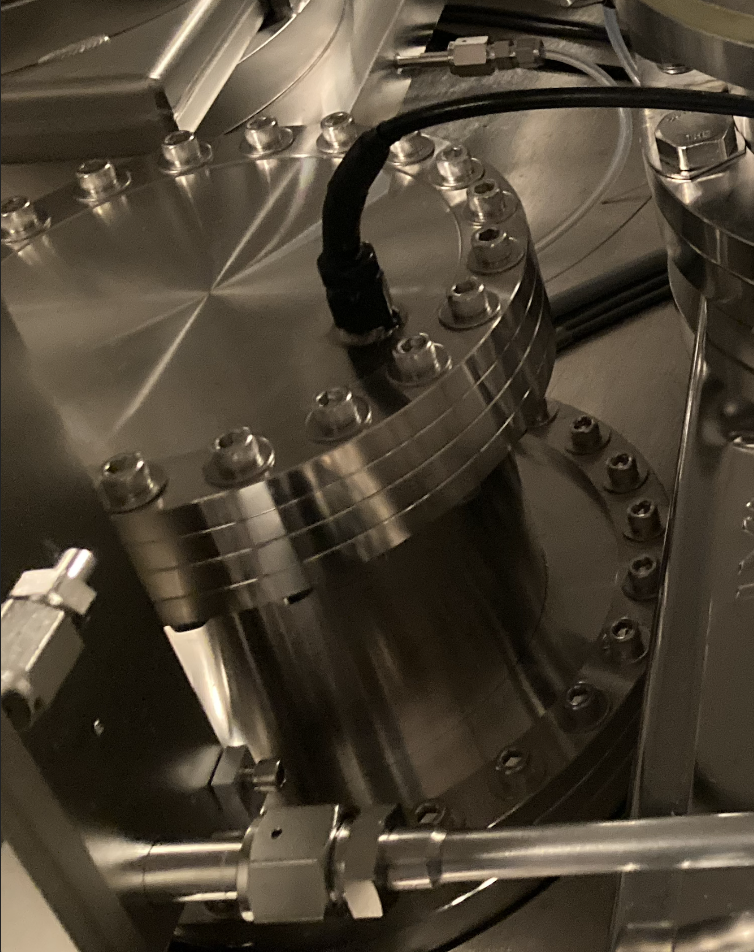
\includegraphics[width=\textwidth]{NeckTubeFeedthrough.png}
	\caption{The Neck Tube feedthroughs.}
	\label{fig:necktubefeedthrough}
	\end{subfigure}
	\begin{subfigure}{0.45\textwidth}
	\includegraphics[width=0.94\textwidth]{BaggedWestNeckTube.png}
	\caption{West neck tube bag}
	\label{fig:necktubebag}
	\end{subfigure}
\caption{Neck tubes feedthroughs are a potential source of radon in the UI that should be evaluated after the motor box seals are remediated.}
\label{fig:necktubes}
\end{center}
\end{figure}

	
\end{document}